\section{Relaxation measurements - Dehmelt method}
\subsection{Set-up and procedure}
\begin{figure}
\centering
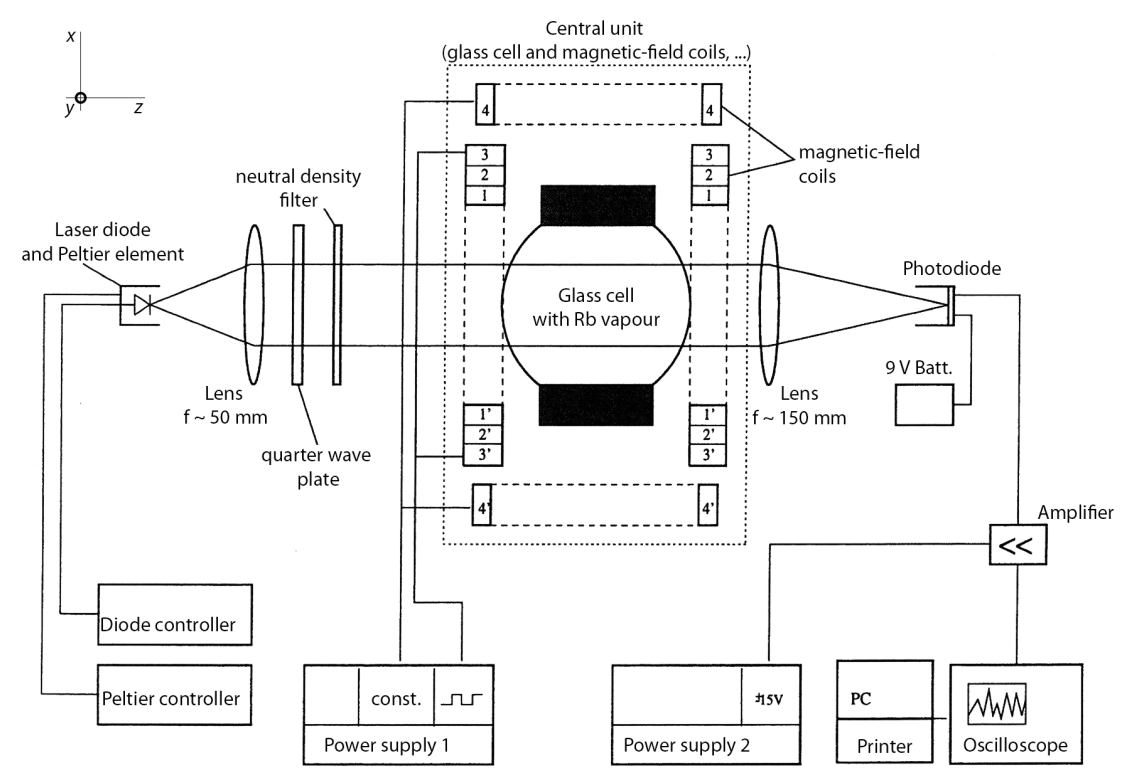
\includegraphics[width=1.0\linewidth]{graphics/dehmeltsetup}
\caption[Set-up relaxation measurements - Dehmelt]{Set-up for the relaxation measurements with the Dehmelt method. A range of neutral filters was used. \cite{anleitung}}
\label{fig:dehmeltsetup}
\end{figure}
If the $^{87}$Rb atoms were in a pumped state, say $F=2$ and $m_F=2$ for example, and the magnetic field responsible for the Zeeman splitting is suddenly reversed, the system is then pumped into the state $F=2$, $m_F=-2$. The measured intensity, after dropping sharply upon reversing the field, increases exponentially until the system is fully pumped. The speed of this process depends both on the laser intensity and speed of relaxation. If one measures this process for various laser intensities, facilitated with neutral filters (see fig. \ref{fig:dehmeltsetup}), the relaxation time $T_R$ of the system can be extracted as it remains constant. For these measurements, the vertical magnetic field will be compensated by coil 4 while coil 3 induces the reversing magnetic field.

\subsection{Data analysis}
All measurements were taken at $T=\unit{34.3}{\degree}$ and a laser current of $I_L=\unit{61.6}{mA}$.\\
As the actual intensity reduction capabilities of the filters were unknown, a calibration measurement of all filters that are later to be used was done. First, a measurement of the intensity without any filter $I_{NF}$ and one of the intensity signal with the laser turned off, $I_0$, were taken. The relative intensity of the former is then set as 1, the one of the latter as 0. The relative intensities for the filter $I^{rel}_F$ are calculated from their absolute measured intensities $I_F$ as
\begin{equation}
I^{rel}_F=\frac{I_F-I_0}{I_{NF}-I_0}
\end{equation}
Table \ref{tb:relintensities} shows the results of these calculations. The errors were calculated through Gaussian error propagation.\\ 
When available, the classification of the filter was used as a name. However, the filter named \emph{triangle} and \emph{circle} did not have a classification written on them, but instead the aforementioned symbols. 

\begin{table}\centering
	\begin{tabular}{@{}lllllll@{}}
		\toprule
		&Filter name&$I_L$ [V]&$I_{rel}$ [\%]&$s_{I_{rel}}$ [\%]&$\tau$ [ms]&$s_\tau$ [ms]\\ 
		\midrule
		&No filter&1.40&100.0&0.8&0.437&0.002\\
		&Triangle&1.11&80.1&0.7&0.503&0.002\\
		&Circle&0.68&50.8&0.6&0.712&0.002\\
		&-0,37&0.55&42.0&0.5&0.859&0.002\\
		&D0,3&0.50&38.5&0.5&0.842&0.002\\
		&0,6&0.48&37.4&0.5&1.121&0.05\\
		&D0,6&0.41&32.2&0.5&0.995&0.005\\
		&D1,0&0.39&31.2&0.5&1.574&0.008\\
		&-0,8&0.17&15.8&0.6&1.602&0.007\\
		&-1,03&0.16&15.2&0.6&2.048&0.023\\
		&D1,3&0.07&8.8&0.6&1.975&0.024\\
		&No laser&-0.06&0.0&0.6&-&-\\
		\bottomrule
	\end{tabular}
	\caption[Relative intensities of the filters]{The relative intensities for the neutral filters. Measurements were only possible for filter until the one marked D1,3.}
	\label{tb:relintensities}
\end{table}

For these filters, measurements of the relaxation times were taken. One such example can be seen in figure \ref{fig:dehmletexample}. Equation \ref{eq:orientationexponential} suggests using an exponential fit to describe the data:
\begin{equation}
I(t)=I_{max}-\Delta I\cdot e^{-a\cdot(t-t_0)}
\end{equation}
where $I_{max}$ is the intensity in the pumped state, $\Delta I$ the amplitude of the change in intensity and $t_0$ is an offset on the time axis to adjust for the fact that the magnetic field was not inverted at $t=0$. The deciding parameter however is $a=1/\tau$, the inverse of the orientation time of the system. The respective values for $\tau$ are listed in table \ref{tb:relintensities}. The values for $a$ can now be plotted against the relative intensities of the filters they were measured with. The result can be seen in figure \ref{fig:inversetaufit}.\\
\begin{figure}
\centering
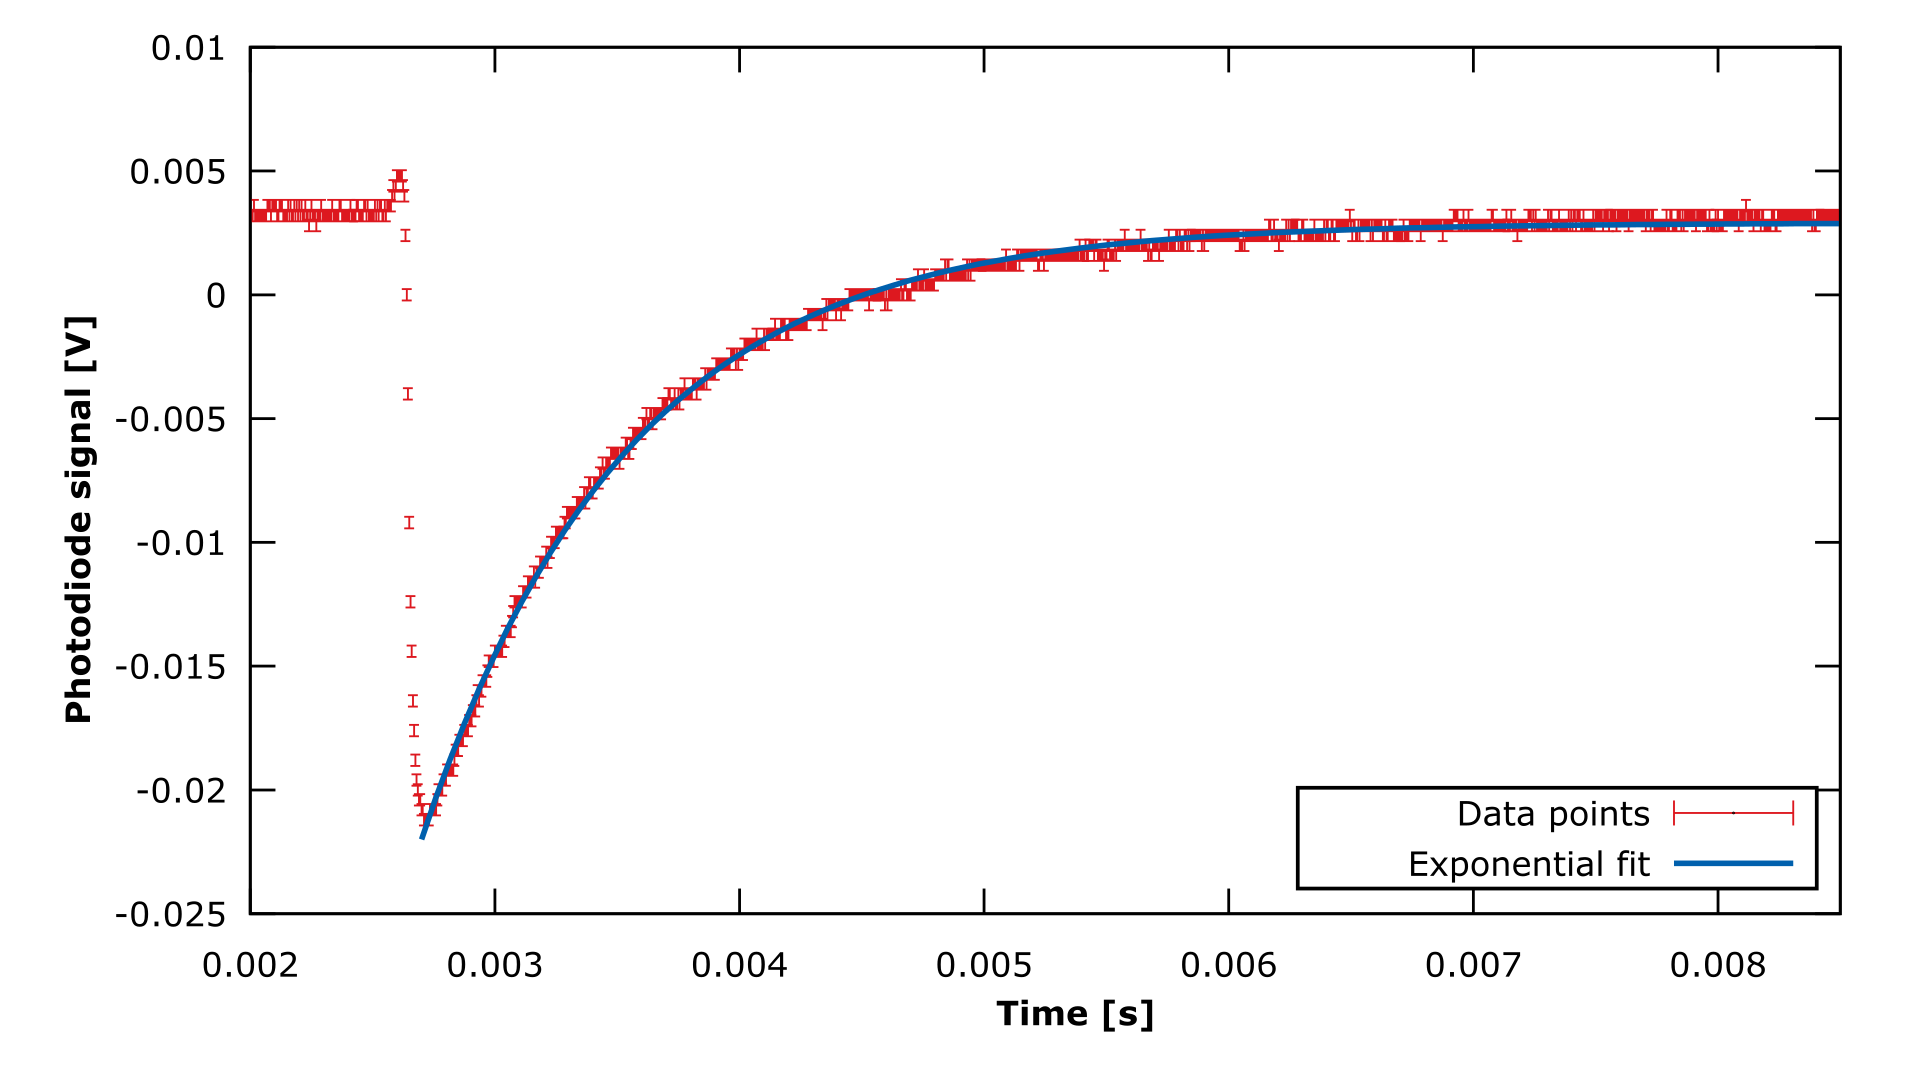
\includegraphics[width=1.0\linewidth]{graphics/dehmletexample}
\caption[Example of Dehmelt relaxation]{Relaxation data recorded with the neutral filter D0,3.}
\label{fig:dehmletexample}
\end{figure}
Equation \ref{eq:tauIrelation} and the fact that the pumping time is inversely proportional to the intensity, $T_P=\frac{1}{\alpha I}$, calls for a fit of the form
\begin{equation}
a(I_{rel})=\alpha I_{rel} + \frac{1}{T_R}
\end{equation}
The values are far more scattered than the uncertainties would suggest. This is expressed in a large $\chi^2\approx105$ as well as in a large error in the desired variable $T_R=\unit{(4.8\pm1.5)}{ms}$. Due to this large error, it includes the expected result of $T_R^{lit}=\unit{6.5}{ms}$ in its $2\sigma$ interval. One likely reason for the larger than expected fluctuation in inverse orientation times would be temperature fluctuations. These have a strong effect on the laser intensity.\\
In the theoretically calculated value, the spin-spin exchange was not taken into account and many calculations were simplified. This might also explain why the measured relaxation time is smaller than predicted.
\begin{figure}
\centering
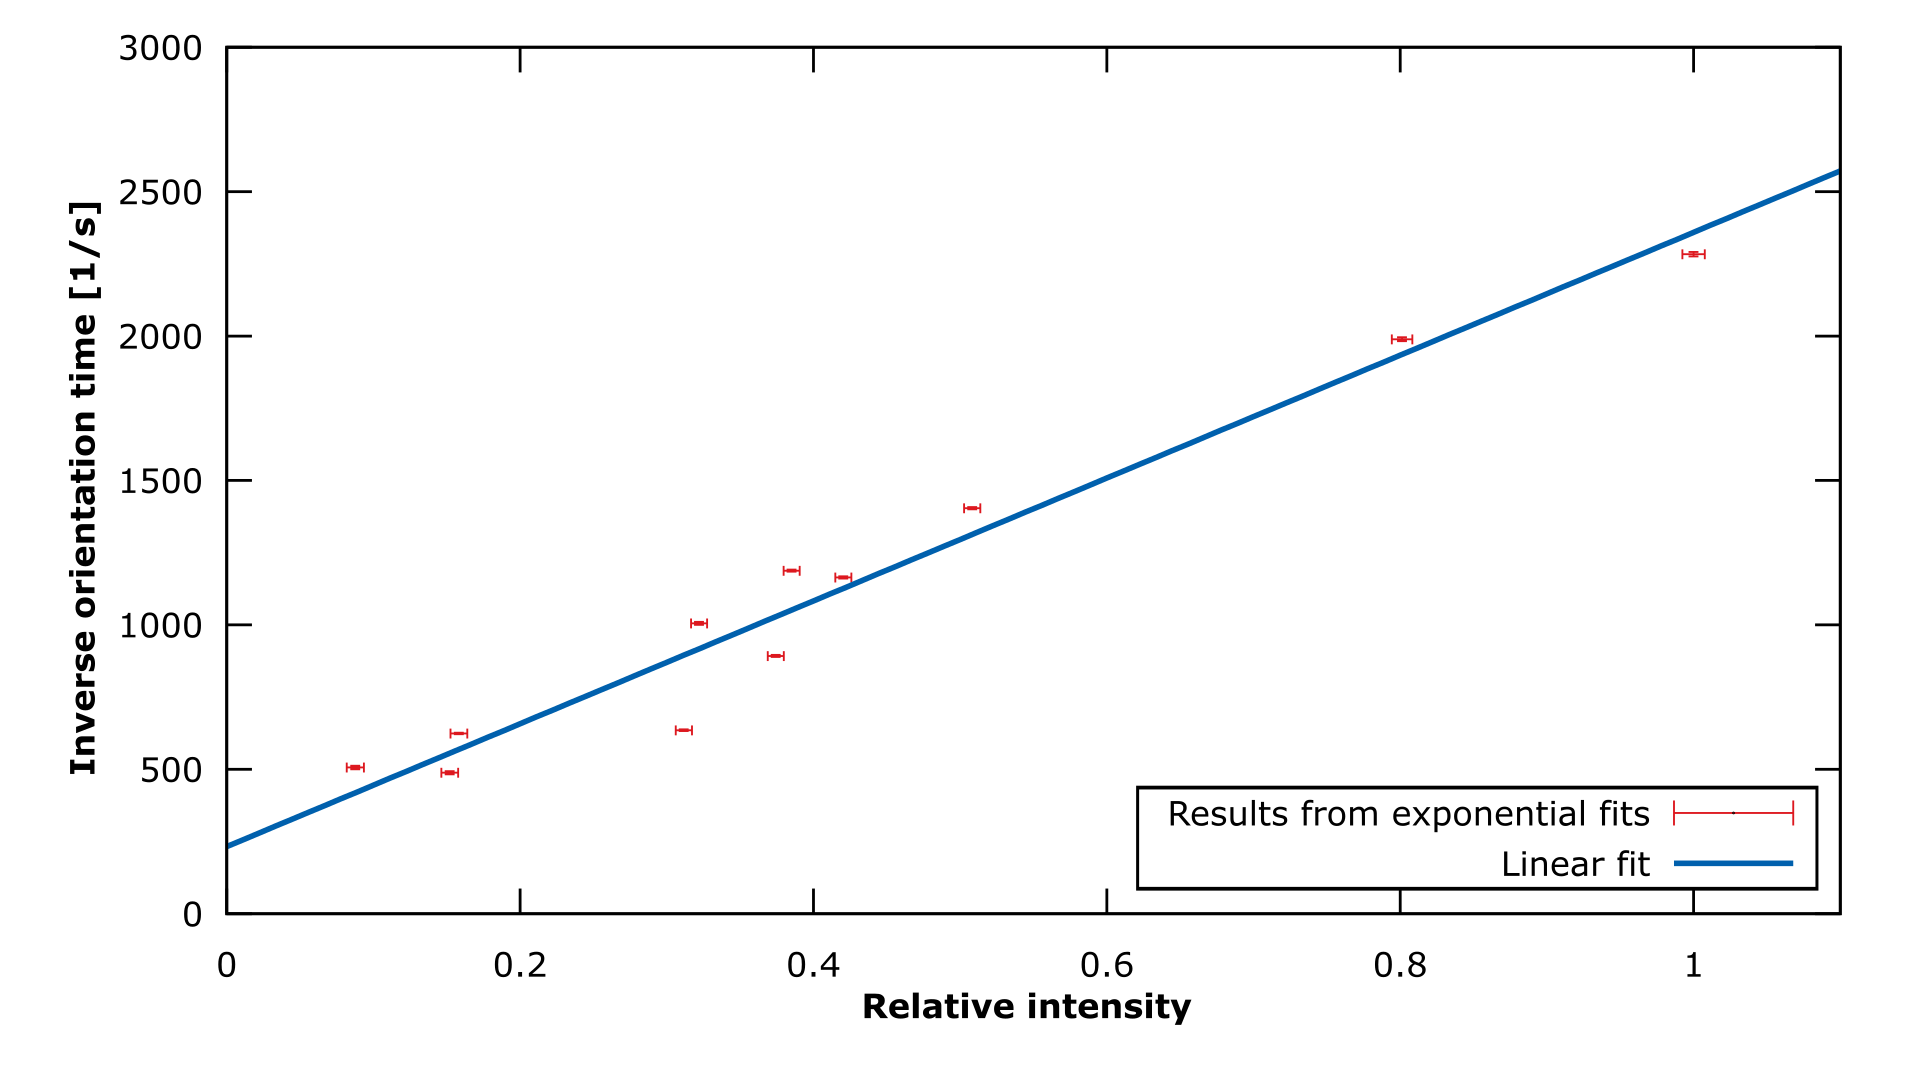
\includegraphics[width=1.0\linewidth]{graphics/inversetaufit}
\caption[Fit on the inverse orientation times]{The fit parameter $a$, which is the inverse orientation time, plotted for the respective relative intensity.}
\label{fig:inversetaufit}
\end{figure}

